\documentclass[pdftex,12pt,a4paper]{report}

\usepackage[portuguese,english]{babel}
\usepackage[T1]{fontenc} 
\usepackage[utf8]{inputenc}
\usepackage[pdftex]{graphicx}
\usepackage{minitoc}
\usepackage{hyperref}
\usepackage{indentfirst}
\usepackage[compact]{titlesec}
\usepackage{fancyhdr}
\usepackage{caption}
\usepackage{pgfplots}
\usepackage{pgfplotstable}
\usepackage{fixltx2e}
\usepackage{mathtools}
\usepackage{fancyhdr}
\usepackage{listings}
\usepackage{color}
\usepackage{sverb}
\usepackage[section]{placeins}

%Highlight
\newcommand{\shellcmd}[1]{\\\indent\indent\texttt{\footnotesize\# #1}\\}

\pagestyle{fancy}
\renewcommand*\thesection{\thechapter\arabic{section}}
\newcommand{\HRule}{\rule{\linewidth}{0.5mm}}
\begin{document}

\begin{titlepage}

\begin{center}


\includegraphics[width=0.15\textwidth]{./logo}\\[0.5cm]    

\textsc{\large Universidade de Aveiro \\[1cm]\large departamento de electrónica, telecomunicações e informática}\\[1cm]

\textsc{\large{47022}\large - Arquitectura de Computadores Avançada \\[1cm]}

\HRule \\[0.5cm]
{ \huge \bfseries  Home group assignment 1}\\[0.4cm]
{ \large \bfseries Implementing a forwarding and stall unit in a pipelined architecture}\\[0.4cm]
\HRule \\[1cm]

\textsc{\small{8240 - MESTRADO INTEGRADO EM ENGENHARIA DE COMPUTADORES E TELEMÁTICA}}\\[1cm]

\begin{minipage}{0.4\textwidth}

\begin{flushleft} \large
\href{mailto:rafael.ferreira@ua.pt}{António Rafael da \\ Costa Ferreira }
 \small{\\NMec: 67405 | P4G1}
\end{flushleft}
\end{minipage}
\begin{minipage}{0.4\textwidth}

\begin{flushright} \large
\href{mailto:rodrigocunha@ua.pt}{Rodrigo Lopes \\ da Cunha}
\small{\\NMec: 67800 | P4G1}
\end{flushright}
\end{minipage}\\[1cm]

{\large Docentes: Nuno Lau/José Luís Azevedo   }\\[0.5cm]

\vfill

{\large Novembro de 2015 \\ 2015-2016}

\end{center}

\end{titlepage} %Titulo do Relatorio
\renewcommand{\headrulewidth}{0pt}

%Cabeçalhos de rodapé
\fancyhead{}
\fancyfoot{}
\lhead{Home group assignment 1}
\rhead{ACA - 2015/2016}
\lfoot{Rafael Ferreira nmec: 67405 \\ Rodrigo Cunha nmec: 67800}
\rfoot{\thepage}

%Renomear Comandos
\renewcommand*\contentsname{Conteúdos}
\renewcommand*\figurename{Figura}
\renewcommand*\tablename{Tabela}

%Conteúdos, dar paragrafo
\tableofcontents
%Headers
\renewcommand{\headrulewidth}{0.15pt}
\renewcommand{\thechapter}{}


\clearpage

\section{Introdução}
% o que, porquê e o objetivo

FALTAAAAAAAAAA

O trabalho proposto para o projeto da unidade curricular de Segurança é um IEDCS: Identity Enabled Distribution Control System. Para o  efeito foi necessário implementar uma Ebook Webstore, um WebService e um Player de reprodução dos Ebooks em formato de texto.

O objetivo deste sistema é garantir a máxima e possível segurança do serviço, utilizando os conhecimentos adquiridos na unidade curricular de Segurança. Para isso são necessários vários processos como por exemplo, a utilização de certificados HTTPS, a cifragem de todo o material existente, derivação de chaves e registo de utilizadores.	

O relatório reflete todos os passos e decisões tomadas na criação do sistema, assim como uma análise ao que foi mostrado na primeira apresentação e decisões que se tomaram depois desta, tecnologias utilizadas, descrição dos vários processos existentes e conclusão.

\newpage
\section{Exercício 1}

\subsection{Divisão da fase ID em duas fases ID1/ID2}
Neste primeiro exercício, era pedido que se fizesse a divisão da fase ID, por duas fases ID1 e ID2.

\begin{figure}[!htb]
\center
 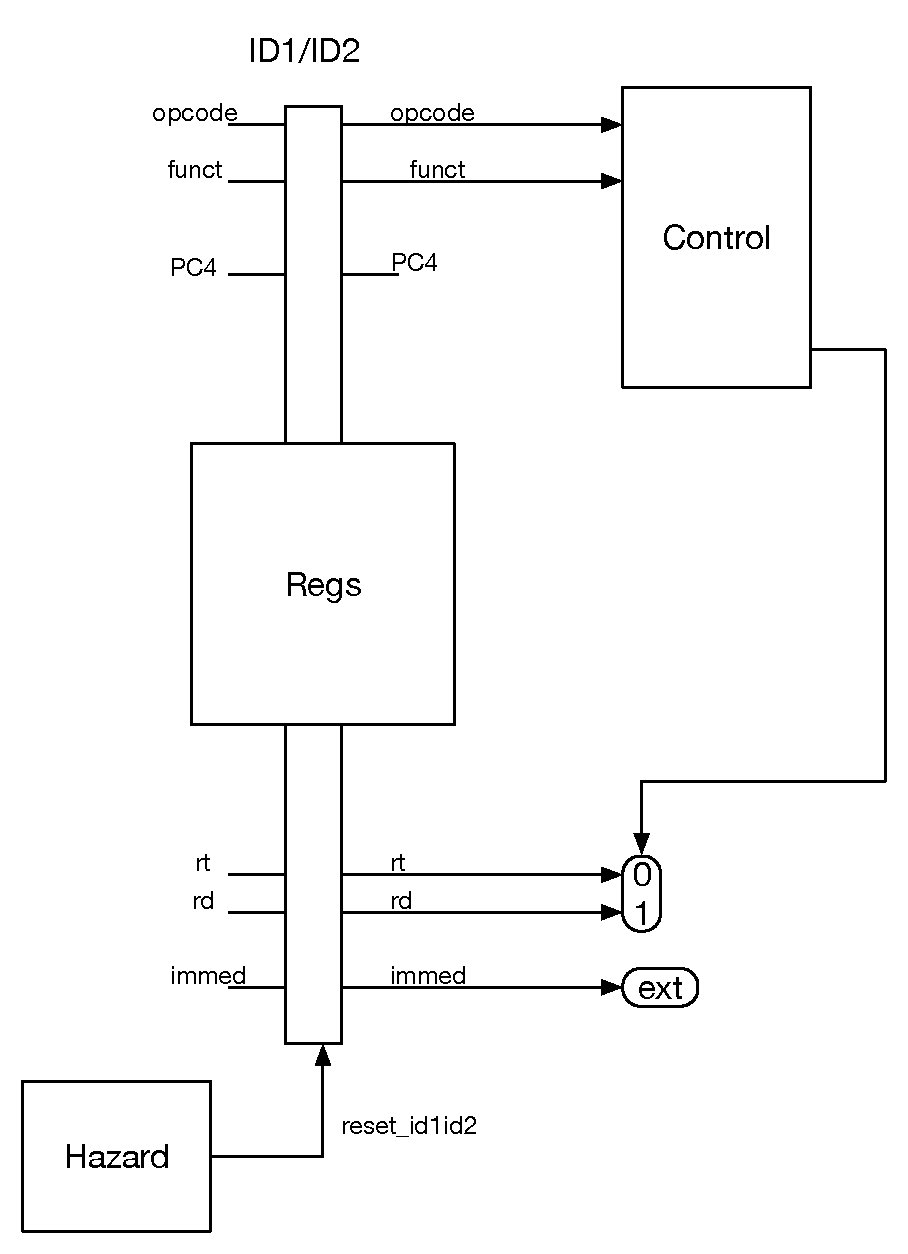
\includegraphics[width=100mm,scale=1]{ID1ID2ex1.pdf}
 \caption{\\ Registo ID1/ID2}
 \label{fig:ex1RegID1ID2}
\end{figure}

O inicio da leitura de registos tem inicio em ID1 e termina em ID2 (como podemos verificar na figura 1), sendo que na fase ID1 também é feito o decode da instrução para obter os sinais de rs, rt, rd, funct, opcode e immed.  Tudo o que se resolvia em ID agora resolve-se em ID2, como por exemplo a unidade de Controlo, o extend e o Mux entre o rt e o rd.

Para este primeiro exercício criou-se um registo novo ID1/ID2, que toma como entradas o \textit{opcode}, o \textit{funct}, o \textit{immed}, o \textit{rt}, o \textit{rs} e o \textit{rd} vindos do decoder de ID1, sendo as saídas as correspondentes a estas mesmas portas. Existe também uma entrada vinda da unidade de Hazard, \textit{reset\_id1id2}, para fazer reset a este registo aquando da necessidade de existirem stalls ou branchs.

Na unidade de hazard foram feitas algumas alterações para que estes fossem resolvidos em ID2, que anteriormente eram resolvidos em ID. A única diferença é que são os registos em ID2, rs e rt, que definem a existência de hazard tendo em conta as fases mais avançadas da pipeline, como EXE, MEM e WB.

\newpage
\section{Exercício 2}

Neste segundo exercício, foi-nos proposto para que todos os saltos condicionais e incondicionais, fossem resolvidos em ID2. Para isso foi criada uma unidade de branch, que através de entradas como \textit{opcode}, \textit{rsdata}, \textit{rtdata}, \textit{branch}, \textit{target}, \textit{imm\_ext} e \textit{PC4}, calcula o \textit{branchTaken}, que nos diz se existe salto ou não, e o \textit{branchTarget} (Figura 2).

\begin{figure}[!htb]
\center
 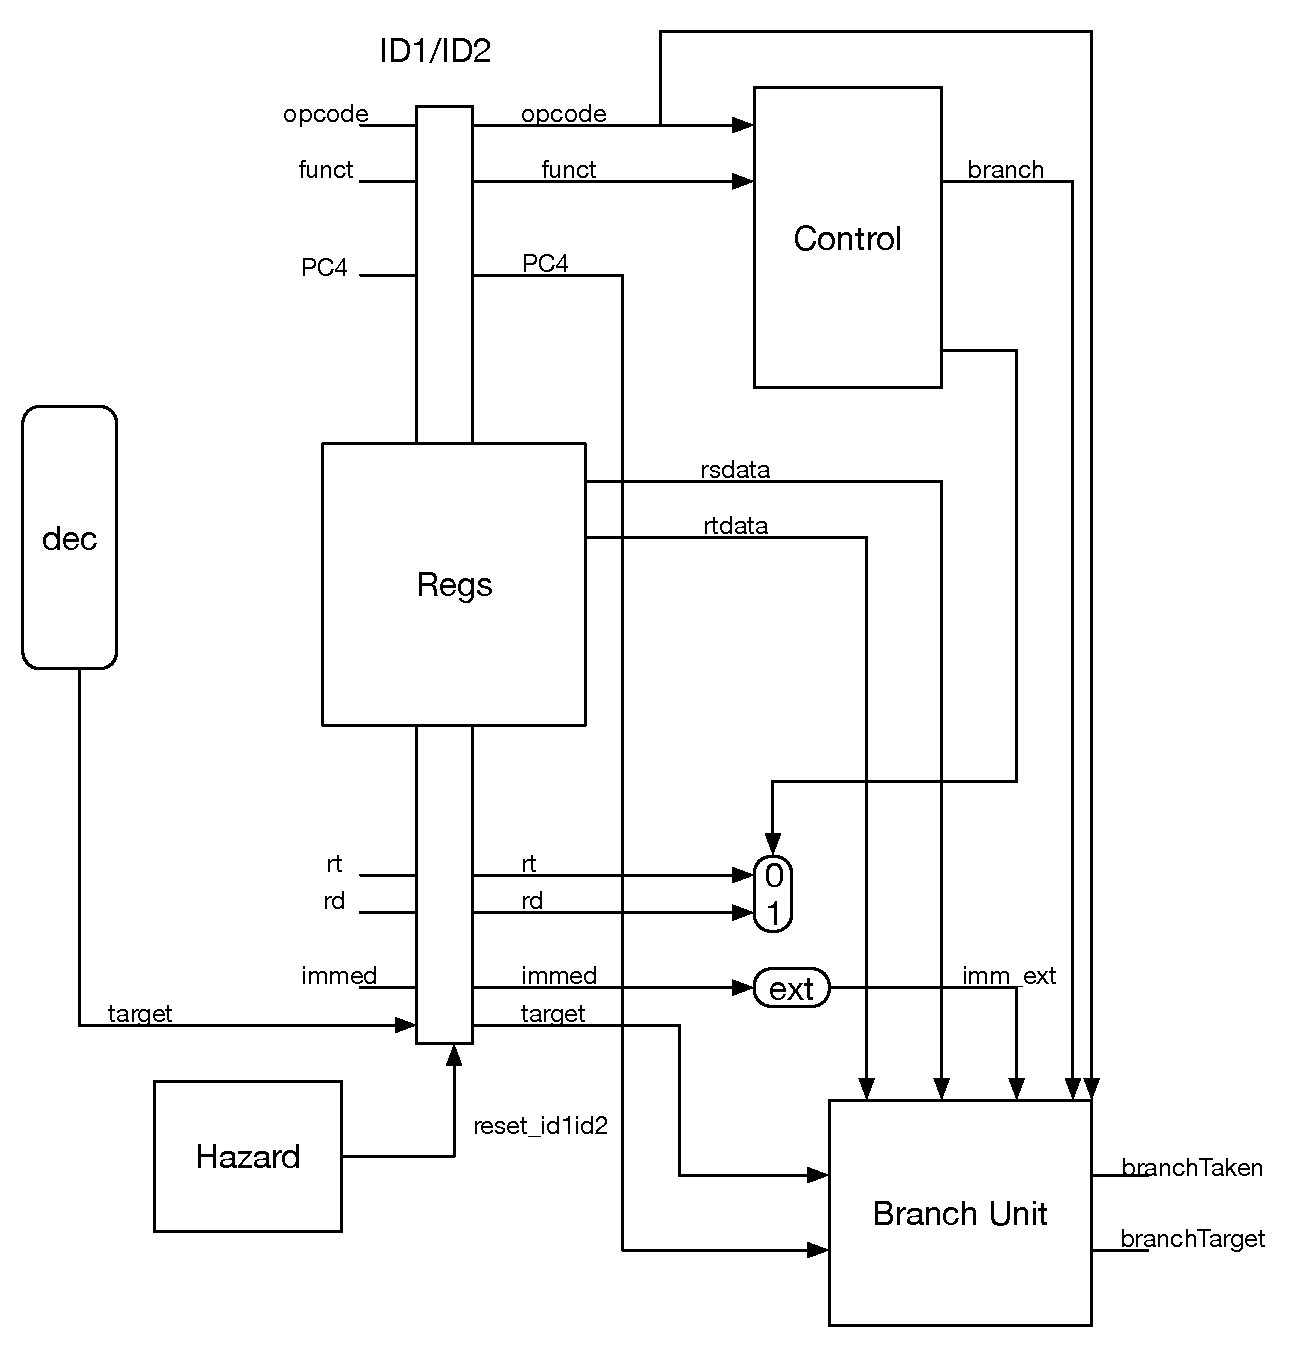
\includegraphics[width=100mm,scale=1]{ID1ID2ex2.pdf}
 \caption{\\Registo ID1ID2 com Branch Unit}\label{fig:ex2RegID1ID2}
\end{figure}

\subsection{Unidade de Branch}

Para que os saltos fossem resolvidos em ID2, foi necessário na unidade de branch resolver os mesmos. Para isto dentro da unidade de controlo, alterou-se a informação que a saída de branch possuí. Disponibilizaram-se mais bits para que esta saída indique na unidade de branch o tipo de salto que estamos a resolver.

Posto isto na unidade de branch, efectuam-se 6 casos diferentes:

\begin{itemize}
\item BEQ: compara se o valor de \textit{rsdata} é igual ao de \textit{rtdata}
\item BNE: compara se o valor de \textit{rsdata} é diferente de \textit{rtdata} 
\item BGTZ: compara se o valor de \textit{rsdata} é maior que zero
\item BLEZ: compara se o valor de \textit{rsdata} é menor ou igual a zero
\item JUMP: salta para o target da instrução
\item JR: salta para o valor de \textit{rsdata}
\end{itemize} 

Sendo os saltos resolvidos em ID2, foram removidos de fases mais avançadas unidades que não seriam mais utilizadas, como por exemplo o \textit{sl2} e a unidade de adição para branch em EXE e o \textit{and} em MEM. Os portos \textit{PC4} e \textit{branch} também deixaram de ser propagados para as fases seguintes à ID2.

\subsection{Unidade de Hazard adaptada para a nova resolução de saltos}

Para que instruções que entrem de forma errada na pipeline quando um branch ocorre sejam descartadas excepto a seguinte (delayed branch slot), foi necessário alterar na unidade de Hazard as fases às quais é necessário fazer reset. Desta feita quando a nossa unidade de Hazard trata de descartar instruções que entrem de forma errada na pipeline e de colocar stalls aquando da ocorrência destes.

\section{Problemas identificados na primeira entrega}


\subsection{Soluções}

\newpage
\section{Conclusão}



\end{document}